\section{Lezione 20}%
\label{sub:Lezione 20}
Possiamo suddividere il caos in due grandi categorie:
\begin{itemize}
    \item Caos Globale: invade lo spazio delle fasi su tutte le scale.
    \item Caos locale: limitato ad una regione dello spazio delle fasi.
\end{itemize}
\subsection{Indicatori di caos locale: esponenti di Lyapunov}%
\label{sub:Indicatori di caos locale: esponenti di Lyapanov}
Intuitivamente una regione è localmente caotica se le traiettorie con condizioni iniziali "vicine" si allontanano "rapidamente" (ed in modo esponenziale).\\
Ci si aspetta che la differenza tra due traiettorie inizialmente vicine venga amplificata esponenzialmente.\\
Quindi possiamo prendere il sistema da studiare, far evolvere due traiettorie con condizioni iniziali vicine e vedere in che modo si allontanano le traiettorie: questa è l'idea alla base degli esponenti di Lyapunov.\\
Definiamo la mappa di partenza come:
\[
    \vect{x}_{n+1} = F(\vect{x}_n)
.\] 
Questa mappa genererà una traiettoria $\vect{x}^{(t)}$. Prendiamo un punto $x_n$ sulla traiettoria $\vect{x}^{(t)}$, vi aggiungiamo una piccola perturbazione $\delta\vect{x}_n$ e andiamo a vedere come evolve la traiettoria.
\[
    \vect{x}_{n+1} + \delta\vect{x}_{n+1} = F(\vect{x}_n) + \frac{\partial F_n}{\partial \vect{x}_n}  \delta\vect{x}_n
.\] 
Quindi si ottiene una evoluzione delle variazioni $\delta\vect{x}_n$ secondo la mappa $F$. Possiamo definire allora la \textbf{mappa tangente} come:
\[
    \delta\vect{x}_{n+1} = \left.\frac{\partial F}{\partial \vect{x}} \right|_{\vect{x}^{(t)}}\delta\vect{x}_n
.\] 
Quindi per ottenere la mappa tangente ci si muove lungo la traiettoria $\vect{x}^{(t)}$  solo che ogni volta si valuta la variazione $\delta\vect{x}_{n+1}$.
\begin{exmp}[Mappa standard]
    \[\begin{aligned}
	&q_{n+1} = q_n + p_{n+1}\\
	&p_{n+1} = p_n + \frac{k}{2\pi}\cos ( 2\pi  q_n)
    .\end{aligned}\]
    In questo caso possiamo fare il seguente cambio di variabili:
    \[\begin{aligned}
	& q_n \to q_n + \delta q_n\\
	& p_n \to p_n + \delta p_n
    .\end{aligned}\]
    A questo punto dobbiamo derivare la mappa rispetto a $q_n$ e $p_n$, in tal modo otteniamo la mappa tangente:
    \[\begin{aligned}
	& \delta q_{n+1} = \delta q_n \\
	& \delta p_{n+1} = \delta p_n - k \sin (2\pi q_n)\delta q_n
    .\end{aligned}\]
    Possiamo scriverla anche in forma di matrice:
    \[
        \begin{pmatrix} \delta q_{n+1} \\ \delta p_{n+1} \end{pmatrix} =
	\begin{pmatrix} 
	    1 & 0 \\
	    -k \sin (2\pi q_n) & 1
	\end{pmatrix} 
	\begin{pmatrix} \delta q_n \\ \delta p_n \end{pmatrix} 
    .\] 
\end{exmp}
\noindent
Quindi per ogni punto della traiettoria $\vect{x}^{(t)}$ abbiamo un set di autovalori ed autovettori che diagonalizzano la mappa tangente ($M$).\\
Ipotizziamo di fare $n$ step della nostra mappa $F$, la mappa tangente varia sotto iterazione nel seguente modo:
\[
    \left(M\right)^{(t)}_n = M(\vect{x}^{(t)}_n)M(\vect{x}^{(t)}_{n-1})\ldots M(\vect{x}^{(t)}_0)
.\] 
Quindi se abbiamo diagonalizzato la mappa tangente alla fine avremo semplicemente che:
\[
    \left(M\right)^{(t)}_n \sim \lambda^n \sim e^{n\ln\lambda}
.\] 
Quindi a questo punto, come già fatto nella lezione precedente, possiamo interpretare $n$ come un tempo e $(\ln\lambda)^{-1}$ il tempo caratteristico del sistema.\\
Notiamo anche che il segno di $\ln\lambda$ decide se le nostre traiettorie divergeranno o rimarranno legate alla traiettoria originale.\\
Visto che vogliamo un oggetto locale e che, alla fine, cerchiamo una quantità che ci dia un "resoconto" di quello che è avvenuto durante la traiettoria consideriamo la radice $n$-esima dell'ultima espressione:
\[
    (M)_n \equiv \left((M^{(t)}_n)\right)^{1/n}
.\] 
Se $D$ è la dimensione del sistema questa equazione avrà $D$ autovalori e $D$ autovettori. L'insieme dei $D$ autovalori si chiama \textbf{Spettro di Lyapunov}: $\sigma_i$.
\[
    \sigma_i = \lim_{N \to \infty} \ln\left|\lambda_i(N)\right| \qquad i = 1, \ldots, D
.\] 
\subsubsection{Spettro di Lyapunov per mappe Hamiltoninane}%
\label{subsub:Spettro di Lyapanov per mappe Hamiltoninane}
Nel caso di un sistema dinamico continuo come quello derivante da una Hamiltoniana in generale si avranno $2n$ esponenti $\sigma$: $n$ per le $p$ ed $n$ per le $q$.\\
In particolare, essendo il sistema Hamiltoninano, devono valere le seguenti proprietà:
\begin{itemize}
    \item $\sum_{}^{} \sigma_i = 0$ per la conservazione del volume nello spazio delle fasi.\\
	Infatti le $\sigma$ ci dicono quanto si espande/contrae il sistema. Se si conserva il volume la somma di tutte queste trasformazioni sarà nulla.
    \item Visto che le variabili $p, q$ sono coniugate si avrà che le $\sigma$ andranno "a coppie": se $\sigma_j=2$ allora esiste $\sigma_{\overline{j}}=-2$. La regola generale si scrive come:
	\begin{equation}
	    \sigma_i = - \sigma_{2n-i+1}
	    \label{eq:20_sigma}
	\end{equation}
	Può sembrare una proprietà non banale, in realtà anch'essa deriva da $dpdq = $ cost.\\
	Come conseguenza di questa regola esisteranno necessariamente due $\sigma$ nulle. \\
	Questo deriva dal fatto che l'Hamiltoniana conserva l'energia, quindi esisterà almeno una curva sul quale giace la traiettoria ad energia zero. Per tale traiettoria si avrà un $\sigma$ nullo, quindi per la \ref{eq:20_sigma} dovranno esistere due autovalori nulli.
\end{itemize}
\subsection{Mappa tangente nel caso unidimensionale}%
\label{sub:Mappa tangente nel caso unidimensionale}
Prendiamo una mappa unidimensionale del seguente tipo:
\[
    x_{n+1} = f(x_n)
.\] 
Quindi la mappa tangente sarà così fatta:
\[
    \delta x_{n+1} = f'\delta x_n = \prod_{J=0}^{} f'_J \delta x_0 
.\] 
Considerando che deve valere: 
\[
    \delta x_{n+1} = e^{N\sigma}\delta x_n
.\] 
L'esponente di Lyapunov per il sistema è:
\[
    \sigma  = \frac{1}{N} \ln\left[\prod_{J=0}^{} f'_J \right] =
    \frac{1}{N}\sum_{J}^{} \ln\left|f'_J\right|
.\]
\begin{exmp}[Esempio unidimensionale]
    \[
        x_{n+1}=2x_n
	\implies
        f'_J = 2
    .\] 
    \[
	\sigma  = \frac{1}{N}\sum_{J}^{} \ln (2) = \ln 2
    .\] 
    Quindi essendo $\sigma >0$ mi aspetto che le traiettorie del moto divergano esponenzialmente al variare dei parametri iniziali, con un tempo tipico dato da $1 /\sigma$.
\end{exmp}
\subsection{Mappa logistica}%
\label{sub:Mappa logistica}
Prendiamo un'altra mappa unidimensionale molto famosa: la mappa logistica.
\[
    x_{n+1}=4\lambda x_n (1-x_n) \qquad 0\le x_n\le 1
.\] 
Il massimo della mappa logistica è per $x = 1 /2$. Ponendo come condizione iniziale $x_0 = 0.5$ ci si accorge che, per avere un moto vincolato tra $\left[0,1\right]$ deve essere $0<\lambda <1$.\\
In questo caso la mappa tangente è:
\begin{equation}
    \delta x_{n+1} = 4\lambda(1-2x_n)\delta x_n
    \label{eq:20_tangente_log}
\end{equation}
Prendiamo ad esempio il caso $\lambda = 3 /4$, possiamo visualizzare la mappa nel piano $x_n$  vs $x_{n+1}$ in figura \ref{fig:figures-20_mappa_logistica_0-75-png}.
\begin{figure}[h]
    \centering
    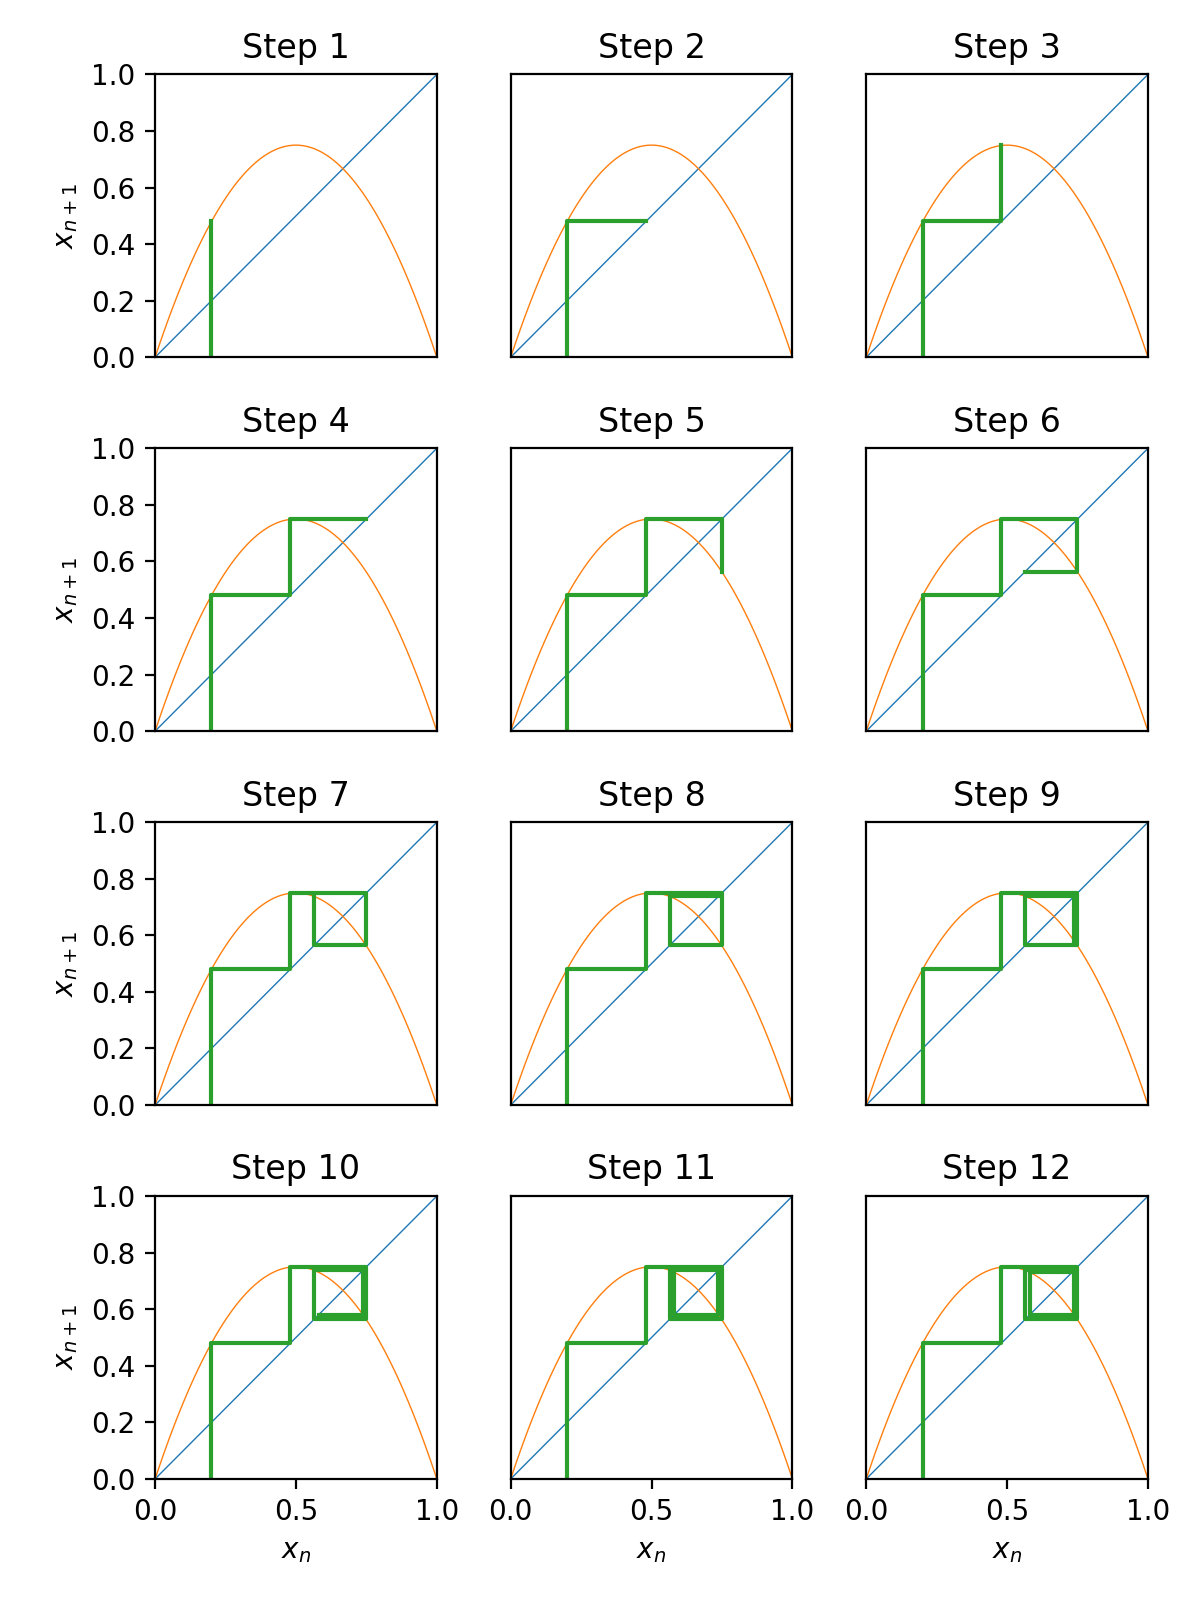
\includegraphics[width=0.45\textwidth]{figures/20_mappa_logistica_0.75.png}
    \caption{\scriptsize Mappa logistica nello spazio $x_n, x_{n+1}$. La linea verde rappresenta la retta tale per cui $x_n = x_{n+1}$, quella arancione invece è il grafico della mappa stessa. \\
    Per costruire gli step è sufficiente proiettare il valore $x_n$ sulla parabola arancione (applicare la mappa) e proiettare $x_{n+1}$ sulla retta verde (mandare $x_{n}$ in $x_{n+1}$). Questi due step vengono ripetuti e rappresentano l'evoluzione della traiettoria.}
    \label{fig:figures-20_mappa_logistica_0-75-png}
\end{figure}
\noindent
Facendo riferimento alla \ref{fig:figures-20_mappa_logistica_0-75-png} i punti in cui la parabola arancione incrocia la retta verde sono punti fissi della mappa. Possiamo notare che una mappa logistica ha due punti fissi: l'origine e quello in alto nel quale la traiettoria sembra girare attorno.
\subsubsection{Stabilità dei punti fissi della mappa logistica}%
\label{subsub:Stabilità dei punti fissi della mappa logistica}
La mappa tangente (\ref{eq:20_tangente_log}) ci aiuta nella valutazione della stabilità dei punti fissi.\\
Partiamo dal punto fisso nell'origine: ponendo $x_n = 0$ nella equazione della mappa tangente:
\[
    \delta x_{n+1} = 4\lambda\delta x_n
.\] 
Quindi se $4\lambda > 1$ l'origine è un punto instabile, viceversa se $4\lambda <1$ l'origine è un punto stabile.\\
L'altro punto fisso si ha imponendo nella equazione della mappa $x_{n+1}=x_n$:
\[
    1 = 4\lambda (1-x_n)
.\] 
\[
    x_n = 1 - \frac{1}{4\lambda}
.\] 
Notiamo che questo oggetto deve essere ancora compreso tra $0$ e $1$, per questo è necessario imporre un vincolo su $\lambda$:
\[
    0 < 1-\frac{1}{4\lambda}<1
.\] 
Quindi deve essere $\lambda >1 /4$.
Inserendo il valore del secondo punto fisso $x_n$ nella mappa tangente:
\[
    \delta x_{n+1}= 4\lambda (1 -2 + \frac{1}{2\lambda})\delta x_n = (-4\lambda  + 2)\delta x_n
.\] 
Quindi ora abbiamo che se $\left|2 - 4\lambda\right| < 1 (> 1)$ abbiamo la (in)stabilità di questo secondo punto fisso.\\
Mettendo tutto insieme:
\begin{itemize}
    \item $\lambda<1 /4$ il punto fisso non c'è.
    \item $1 /4 <\lambda  < 3 /4$ punto fisso stabile.
    \item $3 /4 <\lambda <1$ punto fisso instabile.
\end{itemize}
Possiamo anche raffigurare le traiettorie della mappa al variare del parametro $\lambda$, si ottengono delle immagini molto particolari (figura \ref{fig:figures-20_mappa_logistica_lambda-png}).
\begin{figure}[h]
    \centering
    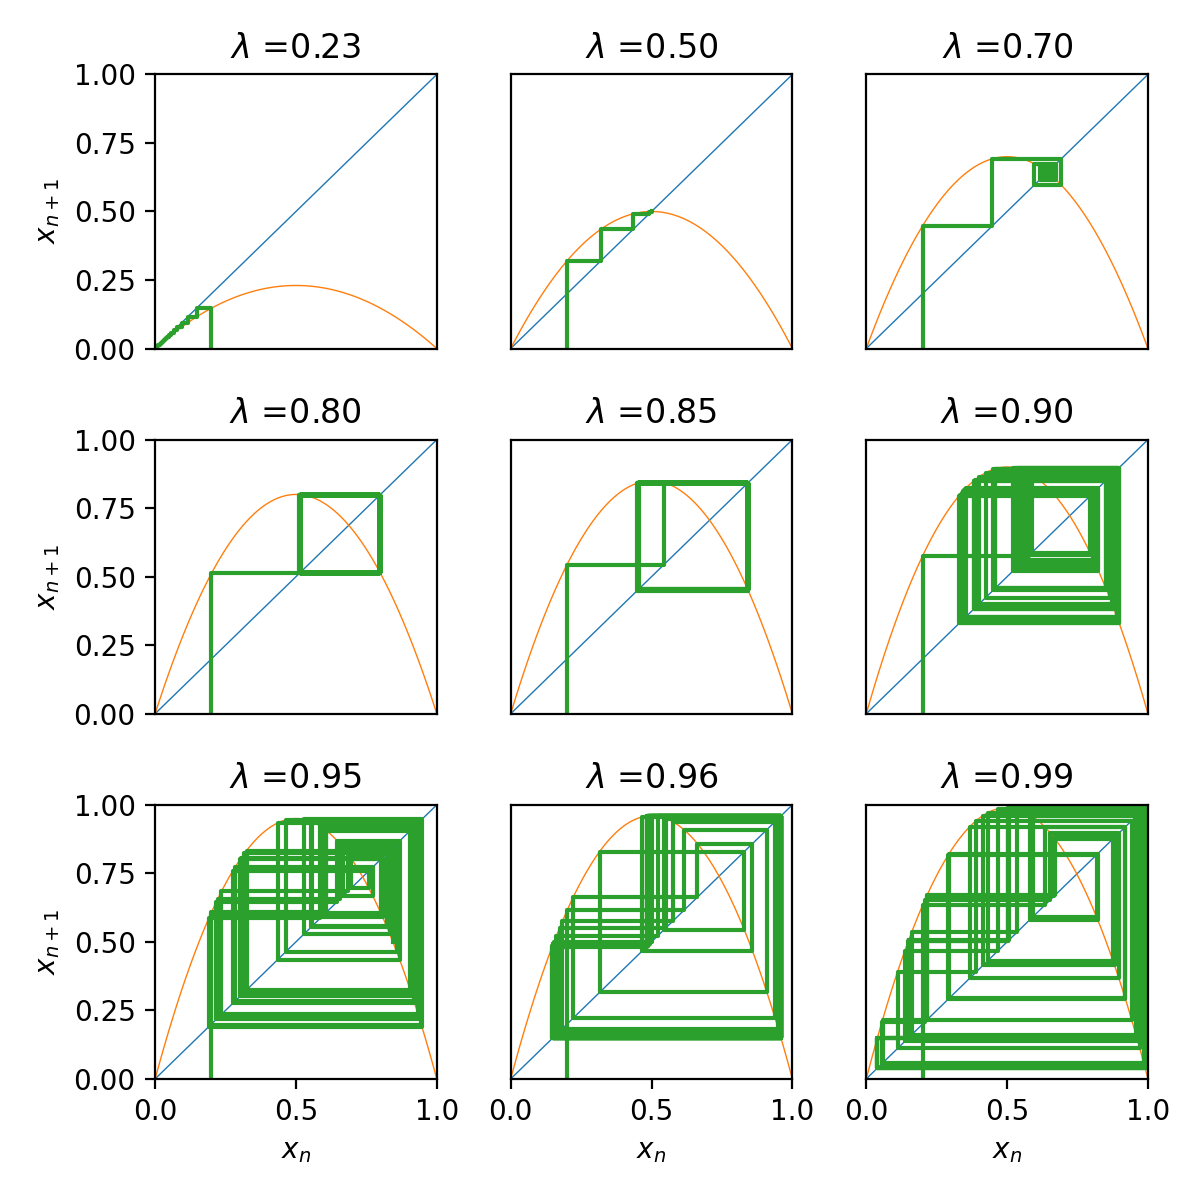
\includegraphics[width=0.45\textwidth]{figures/20_mappa_logistica_lambda.png}
    \caption{\scriptsize Andamento delle prime 100 iterazioni per la mappa logistica al variare di $\lambda$. Dopo un certo valore di $\lambda$ maggiore di $3 /4$ subentra il caos nelle traiettorie.}
    \label{fig:figures-20_mappa_logistica_lambda-png}
\end{figure}
\noindent
Notiamo come, iterando la mappa, se non si sviluppa il caos le traiettorie prediligono pochi punti sul quale adagiarsi. Due dei quali sono (per $\lambda  < 3 /4$) i due punti fissi discussi sopra. \\
Possiamo vedere il subentrare del caos anche con il grafico di Feigenbuam in figura \ref{fig:figures-20_mappa_logistica_-Feigenbuam-png}.
\begin{figure}[H]
    \centering
    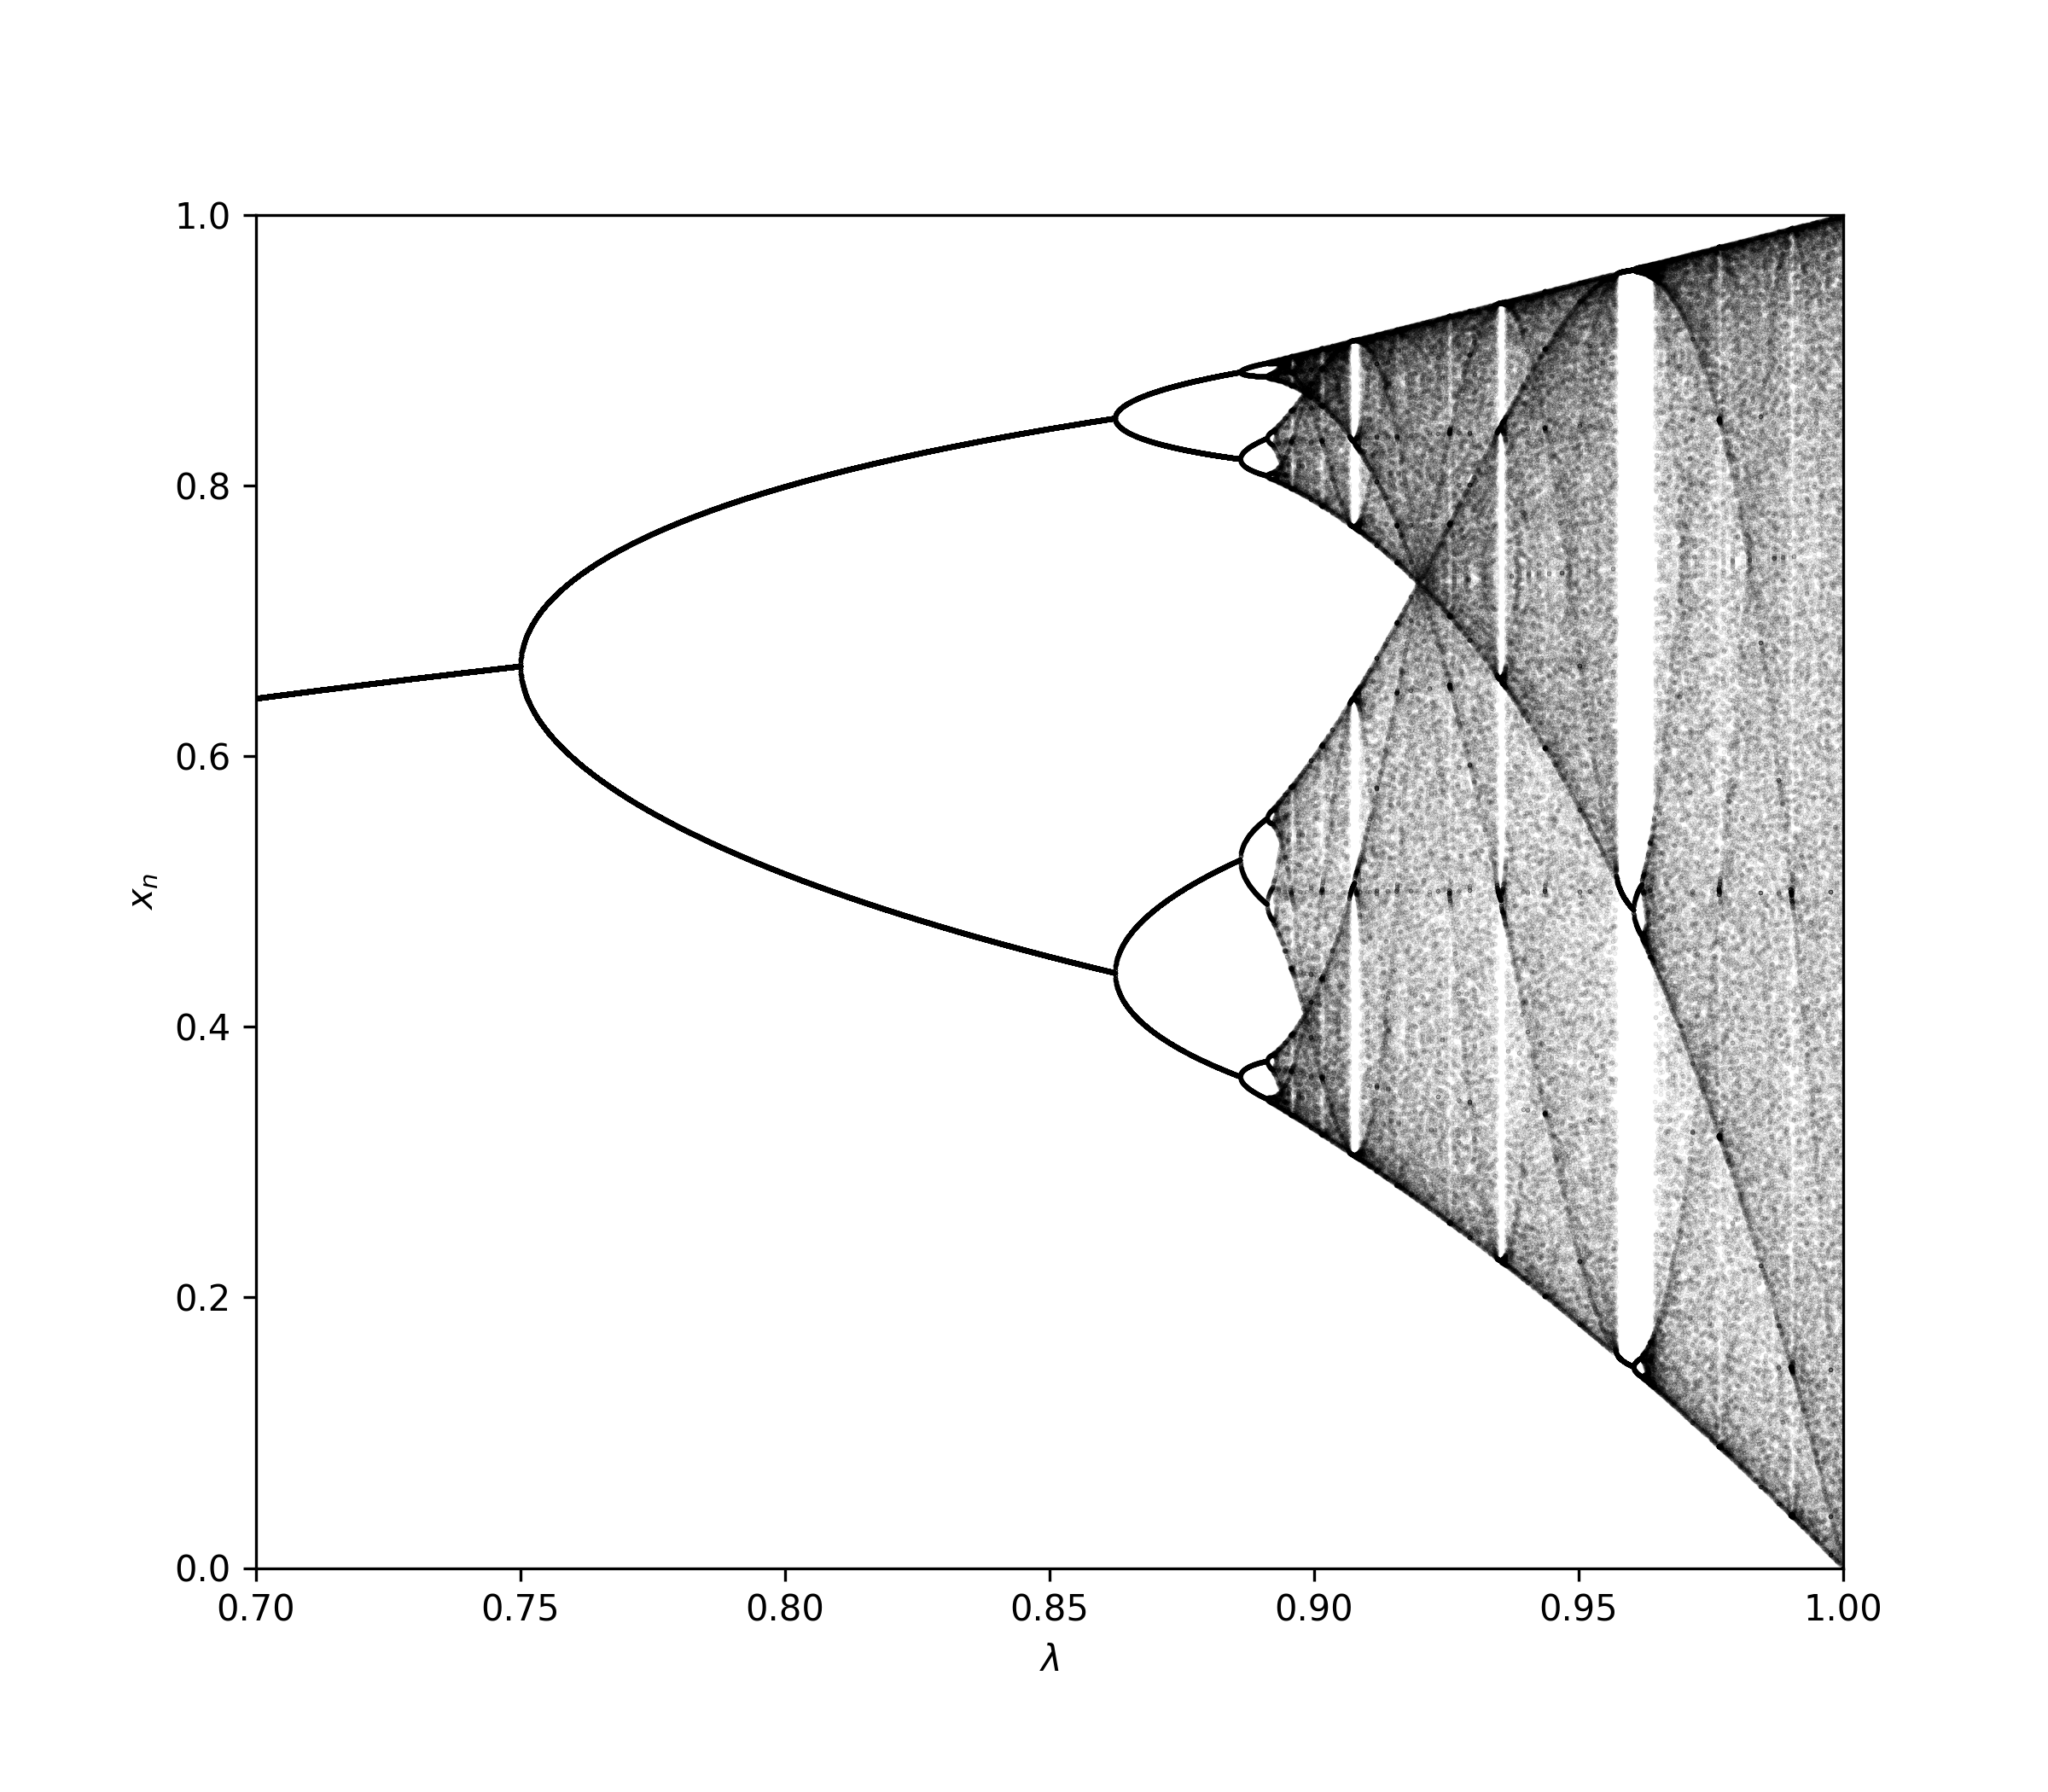
\includegraphics[width=0.5\textwidth]{figures/20_mappa_logistica_ Feigenbuam.png}
    \caption{\scriptsize Andamento degli ultimi 40 step su 20000 al variare di $\lambda$ (i valori che assume $x$ per una traiettoria sono linee verticali). Si nota come dopo qualche diramazione dei valori stabili subentra il caos nella mappa. \\
    La condizione iniziale per ogni traiettoria è $x_0=0.5$.}
    \label{fig:figures-20_mappa_logistica_-Feigenbuam-png}
\end{figure}
\noindent
Questo grafico raffigura gli ultimi valori assunti dalla mappa su un set di $n$ iterazioni. L'idea del grafico è che, dopo un certo tempo, le traiettorie termalizzino su dei punti stabili. Se questo non succede e la mappa si spalma in tutti i possibili valori del dominio allora significa che è subentrato il caos.\\
Si nota come anche per $\lambda > 3 /4$ possano esistere punti attrattori per la mappa. Infatti emergono nel caos delle piccole zone nel quale la mappa assume "pochi" valori. \\
Possiamo anche vedere qual'è l'andamento della media degli esponenti di Lyapunov per la mappa tangente al variare di $\lambda$ in figura \ref{fig:figures-20_mappa_logistica_lyapunov-png}.\\
Si nota subito come, appena prevale il caos nel sistema, gli esponenti siano mediamente positivi. 
\begin{figure}[H]
    \centering
    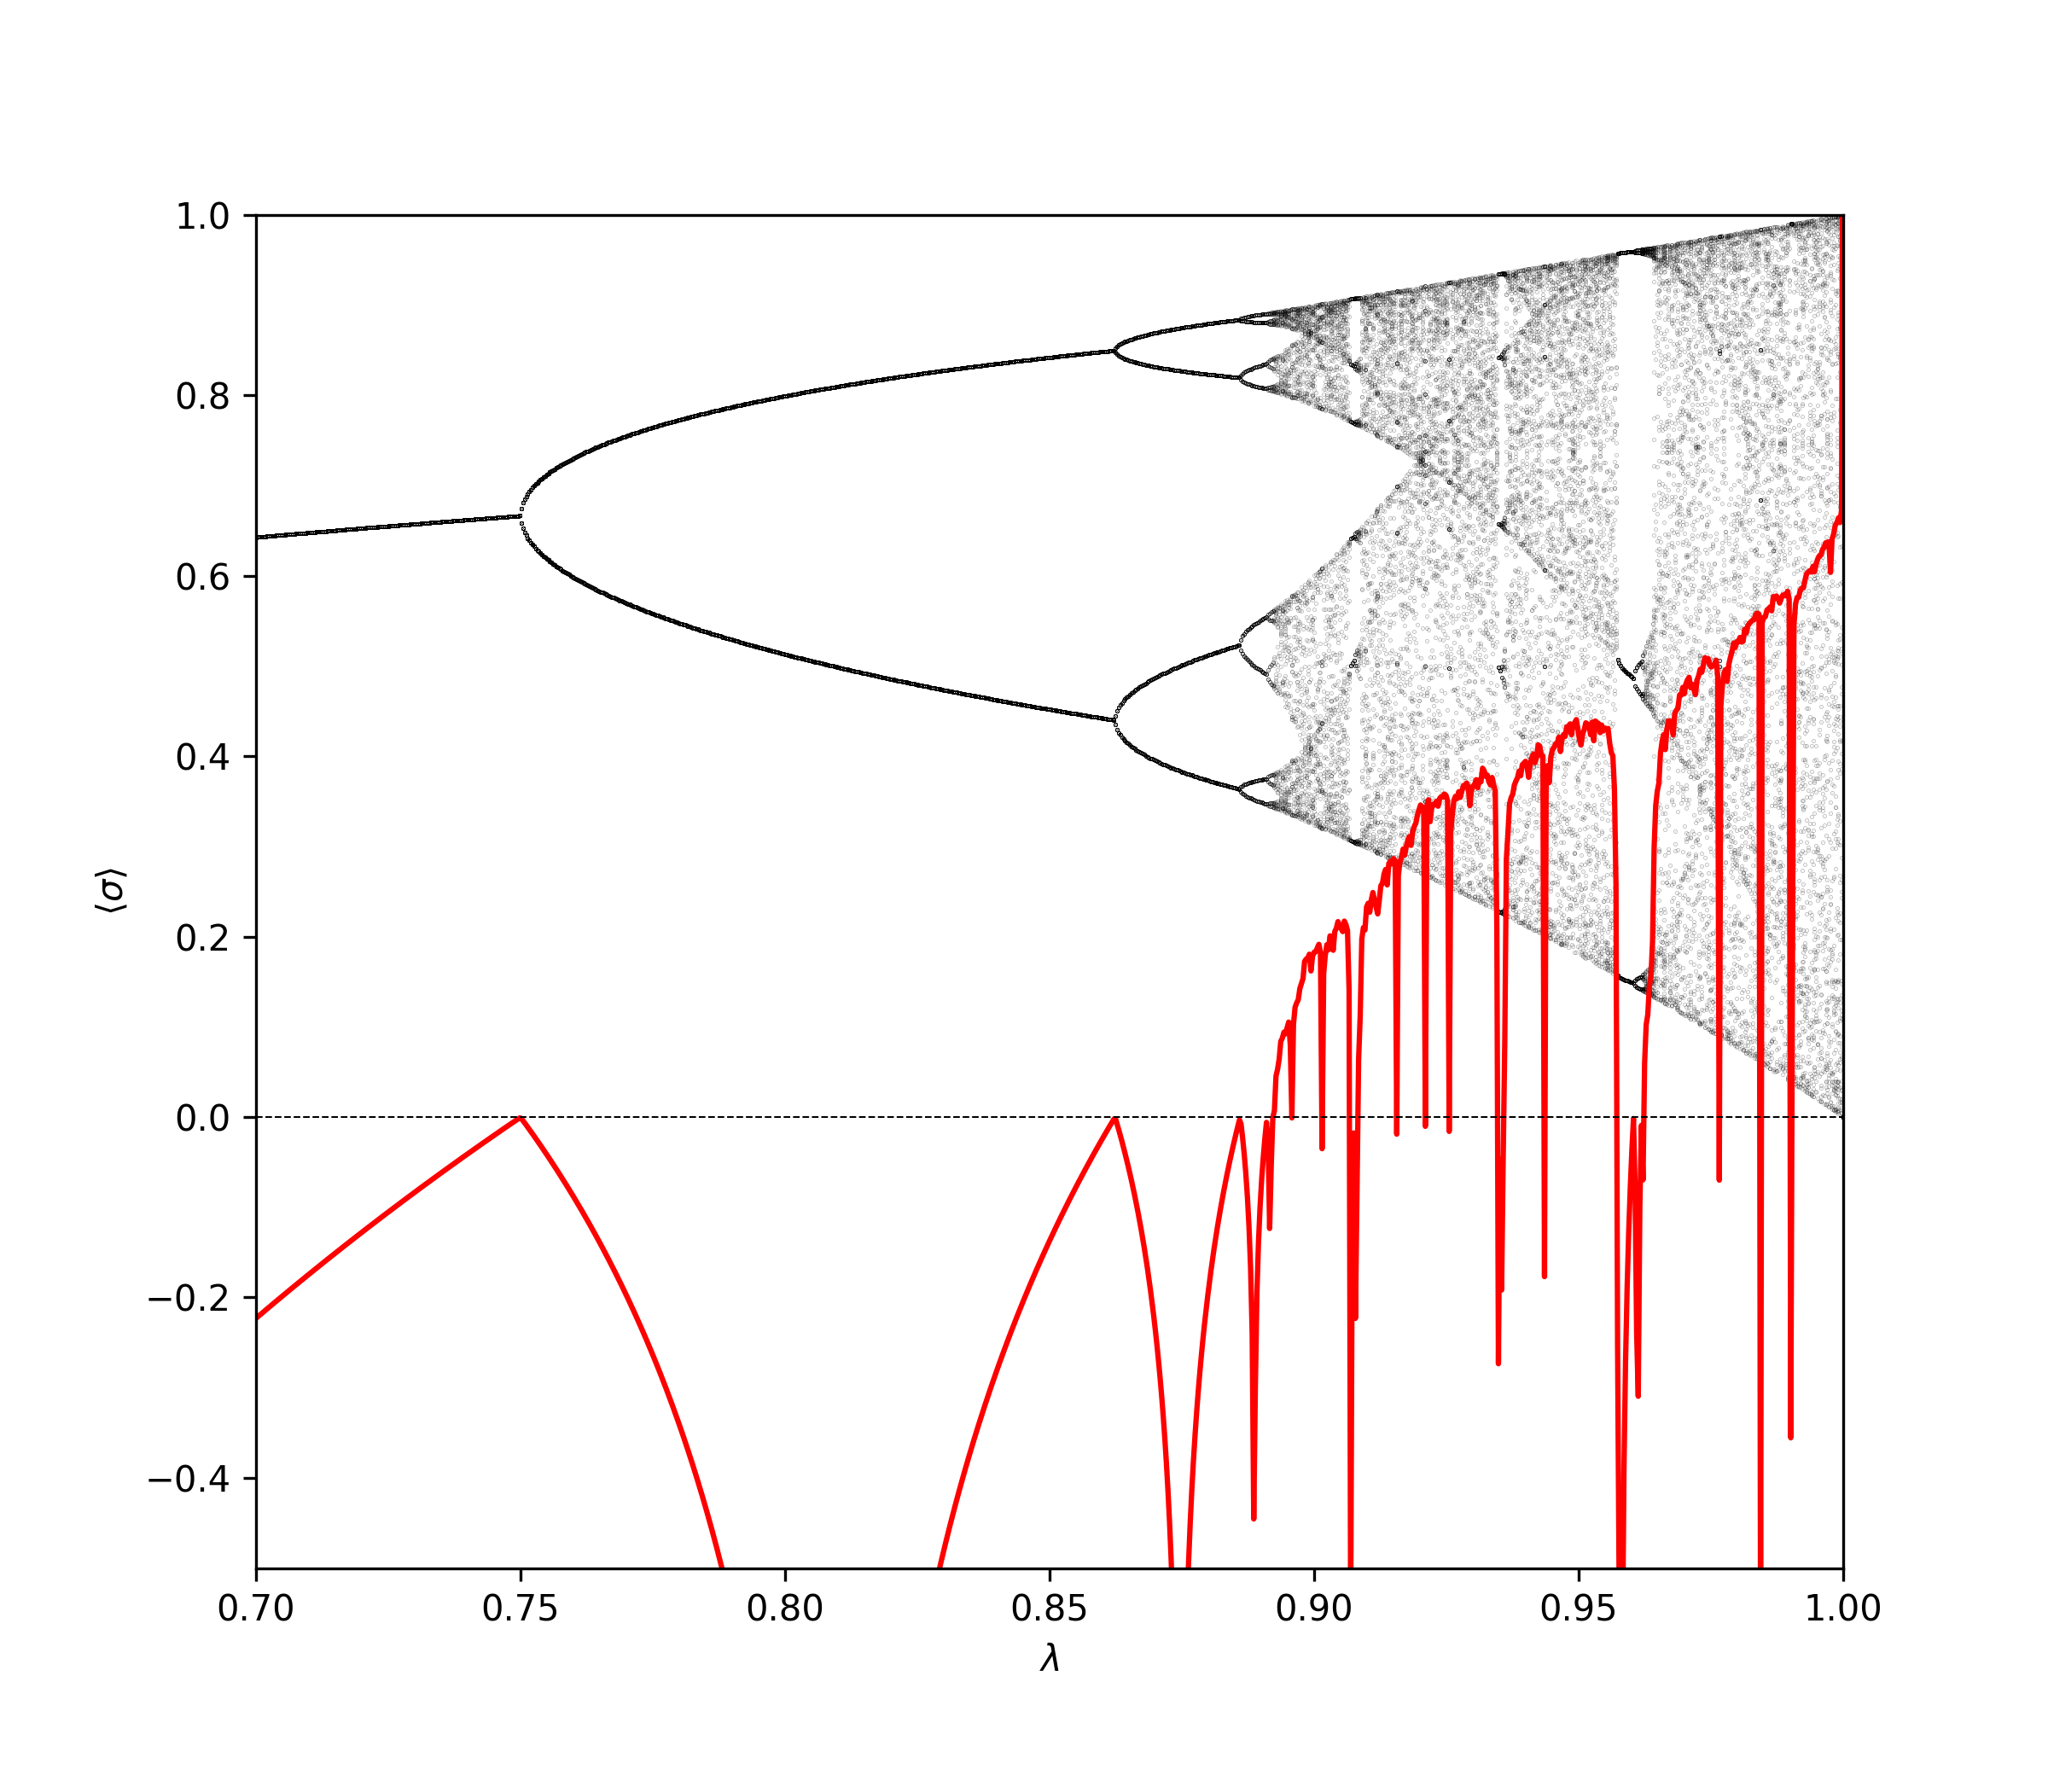
\includegraphics[width=0.5\textwidth]{figures/20_mappa_logistica_lyapunov.png}
    \caption{\scriptsize Andamento della media degli esponenti di Lyapunov al variare del parametro $\lambda$. }
    \label{fig:figures-20_mappa_logistica_lyapunov-png}
\end{figure}
\subsection{Calcolo degli esponenti di Lyapunov in pratica}%
\label{sub:Calcolo degli esponenti di Lyapunov in pratica}
Calcolare gli esponenti di Lyapunov è solitamente molto complicato. Quello che si fa nella maggior parte dei casi è valutare solo il più grande.\\
Infatti non serve valutare ogni esponente: se il più grande è maggiore di $0$ allora possiamo automaticamente dedurre di essere in presenza di un sistema caotico.
\subsubsection{Algoritmo di Benedettin et al. (1976)}%
\label{subsub:Algoritmo di Benedettin et al. (1976)}
La congettura di fondo era di capire da dove venisse fuori il fattore $\hbar $ nella meccanica quantistica. Si ipotizzò che tale valore fosse una soglia al caos: poteva essere che, in un sistema reale, esistesse un valore della azione sopra al quale emergesse il caos, si voleva capire se questo valore fosse parente di $\hbar $.\\
Si parte da una equazione del moto:
\[
    \dot{\vect{x}}=F(\vect{x})
.\] 
Se ne fa la dinamica tangente:
\[
    \frac{\text{d} }{\text{d} t} \delta\vect{x}_i = \sum_{J}^{} \frac{\partial F_i}{\partial X_J} \delta\vect{X}_J
.\] 
Immaginando che la variazione $\delta\vect{x}_i$ (iterata $i$-esima) vada esponenzialmente nel tempo:
\[
    \delta\vect{x}_i(t) \sim e^{\sigma t}\delta x_i(0)
.\] 
Possiamo pensare che questo $\sigma$ sia il valore più grande tra gli esponenti di Lyapunov.\\
Definiamo il modulo delle $\delta\vect{x}_i$:
\[
    d(t)=\sqrt{\sum_{i}^{} \left|\delta x_i(t)\right|^2} 
.\] 
Mi aspetto che anche questa quantità abbia un andamento asintotico con l'esponente di Lyapunov maggiore:
\[
    d(t)\sim e^{\sigma t}d(0)
.\] 
Possiamo allora valutare $\sigma$ nel seguente modo:
\[
    \sigma  = \lim_{\substack{t \to \infty \\ d(0)\to 0}} \frac{1}{t}\ln\left(\frac{d(t)}{d(0)}\right)
.\] 
L'algoritmo operativo prevede di partire con $d(0) = 1$, integrare la mappa con un passo grande $\tau$ e rinormalizzare per ogni step il valore $d(n\tau)$ con $d(0)$. \\
In conclusione si valuta la $\sigma$ come:
\[
    \sigma  = \frac{1}{N\tau}\sum_{J}^{} \ln\left(\frac{d_J}{d(0)}\right)=\frac{1}{N\tau}\sum_{J}^{} \ln\left(d_J\right)
.\] 
\subsubsection{Altri algoritmi per il calcolo di più esponenti di Lyapunov}%
\label{subsub:Altri algoritmi per il calcolo di più esponenti di Lyapunov}
Quando vogliamo calcolare più esponenti di Lyapunov si fa uso dell'algoritmo di Woolf et al.\\
Il problema di questo calcolo deriva dal fatto che, in un sistema Hamiltoniano abbiamo spesso combinazioni di autovalori positivi e negativi. \\
In questi in particolare le variabili sono coniugate è più problematico calcolare gli autovalori in modo preciso.\\
In conclusione siamo sempre in grado di valutare la somma degli autovalori, calcolare il loro valore preciso è molto più complicato.
\clearpage
